\chapter{Introduction}
\label{Introduction}

\begin{quote}
\textit{The dissertation is first presented by contextualizing the scientific background of CERN and LIP organizations, as well as their current research projects, which are closely involved in this work. The motivation for the dissertation is presented in section \ref{Motivation}, with the problem contextualized from a physics perspective in subsection \ref{TopQuarkSystem}. The Goals, subsection \ref{Goals}, states the objectives to be achieved by this work, in terms of improving the research and application development quality by implementing a set of solutions for homogeneous and heterogeneous systems, while assessing the efficiency and usability of hardware accelerators in the latter. The scientific contribution of this work is presented in subsection \ref{ScientificContribution}. Subsection \ref{DissertationStructure} overviews the structure of this dissertation.}
\end{quote}

\section{Context}
\label{Context}

The European Organization for Nuclear Research \cite{CERN} (CERN, acronym for \textit{Conseil Européen pour la Recherche Nucléaire}) is a consorcium of 20 european member countries with the purpose of operating the largest particle physics laboratory in the world. Founded in 1954, CERN is located in the border between France and Switzerland, and employs thousands of scientists and engineers representing 608 universities and research groups and 113 different nationalities.

CERN research focus on the basic constituents of matter, which started by studying the atomic nucleus but quickly moved into high energy physiscs (HEP), focusing on the interaction between particles. The instrumentation used in the nuclear research, physics-wise, is essentially divided into particle accelerators and detectors, alongside with the facilities necessary for delivering the protons to the accelerators. The purpose of the accelerator is to speed up groups of particles close to the speed of light, in opposite directions, and collide them in the detectors (this collision is called an event). The detectors record various characteristics, such as energy and momentum, of particles resultant from complex decay processes of the original particles. These experiments are performed to test and validate specific HEP theories by comparing the results of the collision to the expected theoretical model.

It started with a small low energy particle accelerator, the Proton Synchrotron \cite{CERN:PS} inaugurated in 1959, but the facilities were iteratively being upgraded and expanded. The current facilities are constituted by the older accelerators (some decomissioned while others are still functional) and detectors, as well as the newer Large Hadron Collider (LHC) \cite{CERN:LHC} high energy particle accelerator which is located 100 meter underground and has a 27 km circuference length. There are currently seven experiments running on the LHC: CMS \cite{CERN:CMS}, ATLAS \cite{CERN:ATLAS}, LHCb \cite{CERN:LHCb}, MoEDAL \cite{CERN:MoEDAL}, TOTEM \cite{CERN:TOTEM}, LHC-forward \cite{CERN:LHCf} and ALICE \cite{CERN:ALICE}. Each of these experiments has their own detector on the LHC and conduct similar or different experiments, but with the use of distinct technologies and research approaches. Currently one of the most popular researches being conducted is the validation of the Higgs boson theory. During the next year the LHC will be upgraded to increase its luminosity (amount of energy of the particle beams that it accelerates).
\todo{Fonte disto do upgrade}

Approximately 600 millions of collisions occur every second in each of the experiment's detectors at the LHC, where the detectors react to the particle interaction and produce electric signals, generating massive amounts of raw data. It's estimated that all the detectors combined produce 25 petabytes of data per year \cite{CERN:DATA1,CERN:DATA2}. CERN does not have the financial resources to have the computational power to process all the data, which motivated the creation of the Worldwide LHC Computing Grid \cite{CERN:WLHCCG}, a distributed computing infrastructure that uses the resources of scientific community for data processing. The grid is organized in a hierarchy divided in 4 tiers. Each tier is made by one or more computing centers and has a set of specific tasks and services to perform, such as store, filter, refine and analyse all the data gathered at the LHC.

The Tier-0 is the data center located at CERN. It provides 20\% of the total grid computing capacity, and its objective is to store and reconstruct the raw data gathered at the detectors in the LHC into meaningful information, usable by the remaining tiers. The data is received on a format designed for this reconstruction, with information about detector and software diagnostics. After the reconstruction the data has a different formats, the Event Summary Data (ESD) and Analysis Object Data (AOD), each one with different purposes, containing information of the reconstructed objects and calibration parameters, and can be used for early analysis. This tier distributes the raw data and the reconstructed output by the 11 Tier-1 computational centers, spread among the different countries that are members of CERN.

Tier-1 computational centers are responsible for storing a portion of the raw and reconstructed data and provide support to the grid 24/7. In this tier, the reconstructed data suffers more reprocessing, in order to refine it by filtering only relevante information and reducing the size of the data, now in Derived Physics Data (DPD) format, that is then transferred to the Tier-2 computational centers. The size of the data for an event is reduced from ~3 MB (raw) to ~10 kB (DPD). This tier also stores the outputs of the simulations performed at Tier-2. The Tier-0 center is connected to the 11 Tier-1 centers by high bandwidth optical fiber links, which consists of the LHC Optical Private Network.

There are around 140 Tier-2 computational centers around the world. Their main purpose is to perform Monte-Carlo simulations with the data received from the Tier-1 centers, but also perform a portion of the events reconstructions. The Tier-3 centers range from university clusters to small personnal computers, and they perform most of the events reconstruction and final data analysis. In the CERN related groups terminology, an analysis is a denomination for an application which is designed to process a given amount of data in order to test a specific HEP theory by providing physically relevant information about events that may support the said theory.

\section{LIP Research Group}
\label{LIP}

The Laboratório de Instrumentação e Física Experimental de Partículas (LIP) \cite{LIP} is a portuguese scientific and technical association for research on experimental high energy physics and associated instrumentation. LIP has a strong collaboration with CERN as it was the first scientific organization Portugal has joined, in 1986. It has laboratories in Lisbon, Coimbra and Minho and 170 people employed. LIP researchers have produced several applications for testing various HEP theories of the ATLAS experiment that use Tier-3 computational resources for data analysis. Most of the analysis applications use home-grown frameworks, such as the LipCbrAnalysis and LipMiniAnalysis.

This dissertation work results from a close cooperation between the Department of Informatics of the University of Minho and the LIP laboratory in Minho.

\todo{Falar aqui do que se trata o trabalho ou referir que está explicado mais a frente?}

\section{Motivation, Goals \& Scientific Contribution}
\label{Motivation}

With an increase of events and, consequently, the data being produced by the detectors at the LHC, specifically in the ATLAS experiment, the research groups will need a bigger budget for aquiring and maintaining computational resources due to an increase of analysis to perform. To add up to this data increase, research groups working on the same experiment have a positive rivalry to be the first find and publish relevant results. The finding of these results is directly related to the amount of events processed, meaning that groups with more computational resources are one step ahead.

Better results are not only obtained by increasing the amount of events analyzed; it is important to take into account the quality of each analysis. The ATLAS detector has an experimental resolution of 2\%, meaning that each measured value for a characteristic of a resultant particle of a collision might not be real and, therefore, the analysis will have an error associated. It is possible to improve the analysis quality but it will increase its execution time, creating a trade-off between events to analyze and their quality. This issue will be presented in the context of this dissertation with more detail on subsection \ref{TopQuarkSystem}.

One of the most important analysis being conducted by LIP is related to the Top Quark physics and the Higgs Boson. An application was devised that reconstructs an event following the theoretical model of Top Quark decay and then also attempts to reconstruct the associated Higgs Boson. Each event can be reconstructed several times, with some of its parameters slightly varied by a random offset (with a maximum magnitude of 2\% of the original value), and by chosing the reconstruction that satisfies the most the theoretical model a better solution is obtained, overcoming the experimental resolution of the ATLAS detector. The more reconstructions per event are performed the longer will take to process an event. The theoretical model for this system is presented in subsection \ref{TopQuarkSystem} and the analysis application in chapter \ref{Application}.

While investing in the upgrade of the computational resources of the research group is a valid option to deal with the increase of events to analyze, it is also necessary to take into account if the current resources are being efficiently used by the analysis applications. Also, hardware is not necessarily getting faster, but wider by increasing the number of cores per chip (see chapter \ref{TechnologicalBackground}), which can cause big investments to result in small improvements. Current computing clusters are constituted of systems with one or more multicore CPUs (homogeneous systems) and some even utilizing hardware accelerators, very efficient for specific problem domains (heterogeneous systems). It is important to have a knowledge of these newer architectures in order to develop efficient applications that resort to parallelism in order to better use all the resources available in a system. Programming for such architectures (multicore CPUs and hardware accelerators) requires a set of skills and experience that most physicists (usually self-taught programmers) do not have, causing poorly optimized applications to be developed.

Increasing the efficiency of an application by resorting to parallelism enables the possibility of performing more reconstructions per event and more events to be processed, while using all the potential of the available computational resources and avoiding needless investments in hardware upgrades.

\subsection{The Top Quark system and Higgs boson decay}
\label{TopQuarkSystem}

In the LHC two proton beams are accelerated close to the speed of light in opposite directions, set to collide inside a specific particle detector. From this head-on collision results a chain reaction of decaying particles, from which only some of the final particles react with the detector for recording their characteristics. One of the experiments being conducted at the ATLAS detector is related to the discovery of new Top Quark physics. The schematic representation of the Top Quark decay (the \ttbar system), resulting from a head-on collision of two protons, is presented in figure \ref{fig:TopQuarkDecay}.

\begin{figure}[!htp]
	\begin{center}
		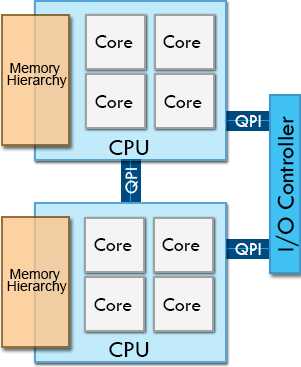
\includegraphics[scale=0.5]{../../common/img/numa_qpi.png}
		\caption{Schematic representation of the \ttbar system.}
		\label{fig:TopQuarkDecay}
	\end{center}
\end{figure}

The ATLAS detector is able to record the characteristics of Bottom Quarks, which are detected as a jet rather than a single particle, and leptons, the muon (that has a positive charge) and electron (with a negative charge). However, the neutrinos do not react with the detector and, therefore, their characteristics are not recorded. To reconstruct the Top Quarks, necessary for researching their properties, it is necessary to have the information of all the final particles, so the neutrino characteristics must be determined. This is possible to do as the \ttbar system obeys a set of properties, and using the information of the quarks and leptons the neutrinos characteristics are analitically calculated. The process of reconstructing the neutrinos is referred as kinematical reconstruction. The reconstruction of the whole \ttbar system has a degree of certainty associated, which determines its quality. The quality of these reconstructions directly affects the quality of the research being conducted by LIP.

The amount of Bottom Quark jets and leptons detected may vary between events, due to other reactions occurring at the same time of the Top Quark decay. As represented in figure \ref{fig:TopQuarkDecay}, it is needed 2 jets and 2 leptons to reconstruct the \ttbar system, but the data for an event may have many of these particles associated. To obtain the best reconstruction for the \ttbar system of a given event it is necessary to reconstruct the respective neutrinos and then the whole system for every combination of 2 jets and 2 leptons, and only chose the most accurate reconstruction.

Another factor affecting the quality of the reconstruction is the experimental resolution of the ATLAS particle detector, which associates an error of 2\% with every measurement made. If the measurements of the jets and leptons are not precise enough the kinematical reconstruction will produce inaccurate neutrinos and affect the overall reconstruction of an event, which might render an event with relevant physics useless. It is possible to overcome this problem by performing the kinematical reconstruction, and then the whole \ttbar system reconstruction, a large amount of times for each combination of 2 Bottom Quark jets with 2 leptons, with a random variation to the particle characteristics (momentum, energy and mass) of a maximum magnitude of 2\% of the original value. The amount of variations performed per combination will directly impact the final quality of the event reconstruction, as more of the search space (defined by the experimental resolution error) is covered compared to performing a single reconstruction. The more variations are performed the more likely it is to find the best possible reconstruction of the \ttbar system.

The look for the Higgs Boson is also part of the research being conducted at LIP. Figure \ref{fig:HiggsBosonDecay} schematizes the Higgs Boson and Top Quark decay. It is possible to reconstruct the Higgs Boson from the two Bottom Quark jets that it decays to, and it can be performed alongside the \ttbar system reconstruction. This adds at least two more jets to the event information, and it is not possible to know before the reconstruction which jets belong to the Higgs decay or the Top Quark decay. Considering this, the Higgs reconstruction must be performed after the \ttbar system reconstruction, in such a way that the jets chosen to reconstruct it must not be the ones used in the \ttbar system reconstruction. Adding this new jets increases the number of jets/leptons combinations to test in the kinematical reconstruction, and for each \ttbar system reconstruction the Higgs must be also reconstructed. Now, the quality of the event reconstruction depends on the quality of both \ttbar system and Higgs Boson reconstructions.

\begin{figure}[!htp]
	\begin{center}
		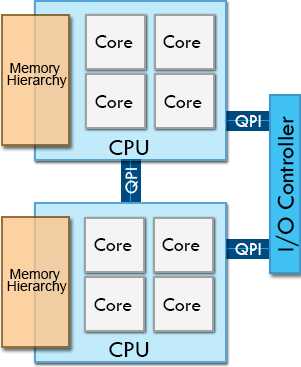
\includegraphics[scale=0.5]{../../common/img/numa_qpi.png}
		\caption{Schematic representation of the \ttbar system with the Higgs Boson decay.}
		\label{fig:HiggsBosonDecay}
	\end{center}
\end{figure}

This specific analysis of events presented is performed by an application developed by LIP researchers, the \tth. The application receives input data file with a set of events and reconstructs the \ttbar system and the Higgs Boson for each event using the processes described. These files are usually 1 GB long and the LIP research requires that hundreds of them are processed by the same application, considering a specific experiment such as the presented in this subsection. A in-depth computational analysis of \tth is presented in chapter \ref{Application}, where its flow is presented, it is characterized in terms of various metrics (such as computational intensity) and the critical regions are identified.

\subsection{Goals}
\label{Goals}

By increasing the performance of the Top Quark and Higgs Boson reconstructions it is possible to perform more variations per event, increasing the quality of the results, and increase the throughput of events processed. The objective of this dissertation work is to take a sequential application made by physicists, which the main concern during its development was the correcteness of the code rather than its performance, the \tth, and improve its efficiency by (i) identifying the bottlenecks and optimizing the code, (ii) increasing the performance by resorting to parallelism for homogeneous and heterogeneous systems, assessing the efficiency (performance and usability) of hardware accelerators for this type of problem, and (iii) the development of a simple scheduler for managing the workload among various instances of the same sequential or parallel application (i.e. an application which needs to process a large set of separate input files) on homogeneous systems.

This work will give a inside perspective of how scientific applications are being developed by programmers with little to no background in computer science, and possibly define a set guidelines for coding of efficient applications and the usage of parallelism in such applications. All the changes that will be made to the \tth application, including the introduction of parallelism, will be as independent as possible from the context of this specific problem, in such a way that they might be portable to other applications without requiring major modifications. The work will be structured, implementation wise, so that the parallelization mechanisms and the scheduler are possible to be improved and transformed in a tool used by the researchers at LIP.

\subsection{Scientific Contribution}
\label{ScientificContribution}

This dissertation work aims to improve the quality of a specific research field conducted by LIP, provide a set of tools and know-how to improve the performance of similar scientific applications and expose the problematic of unefficient usage of computational resources. By improving the quality of the research, LIP will gain an advantage over other research groups in the look for new Top Quark physics and in the Higgs Boson discovery. By experiencing the process of optimizating scientific applications of this kind it is possible to provide physicists with some know-how and tools for optimization and parallelization with the goal of increasing the performance in future applications. By developing applications that efficiently use all the computational resources available it is possible to reduce the investment in new hardware, which otherwise would have small pratical returns.

\section{Dissertation Structure}
\label{DissertationStructure}

This dissertation has 5 chapters and their summary is presented below:

\begin{description}
	\item[Introduction] \hfill \\
	The dissertation is first presented by contextualizing the scientific background of CERN and LIP organizations, as well as their current research projects, which are closely involved in this work. The motivation for the dissertation is presented in section \ref{Motivation}, with the problem contextualized from a physics perspective in subsection \ref{TopQuarkSystem}. The Goals, subsection \ref{Goals}, states the objectives to be achieved by this work, in terms of improving the research and application development quality by implementing a set of solutions for homogeneous and heterogeneous systems, while assessing the efficiency and usability of hardware accelerators in the latter. The scientific contribution of this work is presented in subsection \ref{ScientificContribution}. Subsection \ref{DissertationStructure} overviews the structure of this dissertation.
	\item[Technological Background] \hfill \\
	This chapter presents the current technological state of the art in terms hardware and software. Hardware-wise, both homogeneous and heterogeneous system architectures and details are presented in sections \ref{HomogeneousSystems} and \ref{HeterogeneousSystems}, respectively. A contextualization of current hardware accelerators is also made in the latter. Software-wise is presented in section \ref{Software}. Various frameworks and libraries are presented for homogeneous systems and accelerators in sections \ref{pThreads}, \ref{OpenMP}, \ref{MPI} and \ref{CUDA}. Section \ref{HeterogeneousFrameworks} presents the available frameworks for parallelization in heterogeneous systems. Finally, current solutions for profiling and debugging parallel applications is presented in section \ref{ProfilingDebugging}.
	\item[\tth Application] \hfill \\
	The \tth application for event reconstruction is presented in this chapter. Its dependencies are presented. The flow of the application is presented in section \ref{Application:Flow}, accompanied by a schematic representation. Its main functions are presented and the schematic flow is compared against a callgraph of the application to help understanding what happens in each of the most important functions. The critical region is identified in section \ref{CriticalRegion} and characterized in subsection \ref{ComputationalCharactrization}. Some initial optimizations to the code are presented in subsection \ref{InitialOptimizations}.
	\item[Parallelization Approaches] \hfill \\
	For different parallelization alternatives are presented in this chapter. For homogeneous systems, a shared memory parallelization is discussed in section \ref{Parallelization:SharedMem}, where the abstract heuristic used is shown, and the implementation and a performance analysis are presented in subsections \ref{SharedMemImplementation} and \ref{SharedMemPerformance}, respectively. For heterogeneous systems using hardware accelerators, two alternatives are presented: using GPU as an accelerator, in section \ref{Parallelization:GPU}, with its implementation and performance discussed and analyzed in subsections \ref{GPUImplementation} and \ref{GPUPerformance}; using the \intel Xeon Phi as an accelerator in section \ref{Parallelization:MIC} and its implementation discussed in subsection \ref{MICImplementation}. A software scheduler for managing workload distribution among applications for homogeneous shared memory systems is presented in section \ref{Parallelization:Scheduler}. Its implementation details and performance analysis are shown in subsections \ref{SchedulerImplementation} and \ref{SchedulerPerformance}.
	\item[Conclusions \& Future Work] \hfill \\
	This chapter concludes the dissertation, presenting an overview of the results obtained by the work developed, on both homogeneous and heterogeneous systems. Guidelines for future work, on improving the test case application and providing parallel solutions abstracted from the programmer for future application development, are presented.
\end{description}
